%%%%%%%%%%%%%%%%%%%%%%%%%%%%%%%%%%%%%%%%%
% Beamer Presentation
% LaTeX Template
% Version 1.0 (10/11/12)
%
% This template has been downloaded from:
% http://www.LaTeXTemplates.com
%
% License:
% CC BY-NC-SA 3.0 (http://creativecommons.org/licenses/by-nc-sa/3.0/)
%
%%%%%%%%%%%%%%%%%%%%%%%%%%%%%%%%%%%%%%%%%

%----------------------------------------------------------------------------------------
%	PACKAGES AND THEMES
%----------------------------------------------------------------------------------------

\documentclass{beamer}

\usepackage[utf8x]{inputenc}
\usepackage[T1]{fontenc}
\usepackage{lmodern}
\usepackage[romanian]{babel}
\usepackage{amsmath}
\usepackage{listings}



\mode<presentation> {

\usetheme{Frankfurt}
\usecolortheme{dolphin}

%\setbeamertemplate{footline} % To remove the footer line in all slides uncomment this line
%\setbeamertemplate{footline}[page number] % To replace the footer line in all slides with a simple slide count uncomment this line

\setbeamertemplate{navigation symbols}{} % To remove the navigation symbols from the bottom of all slides uncomment this line
}

\usepackage{graphicx} % Allows including images
\usepackage{booktabs} % Allows the use of \toprule, \midrule and \bottomrule in tables

%----------------------------------------------------------------------------------------
%	TITLE PAGE
%----------------------------------------------------------------------------------------

\title[Cuckoo Hashing]{Algoritmi de hashing de complexitate O(1) Cuckoo Hashing} % The short title appears at the bottom of every slide, the full title is only on the title page

\author{Vlad-Doru Ion} % Your name
\institute[UNIBUC] % Your institution as it will appear on the bottom of every slide, may be shorthand to save space
{
Universitatea din București \\ % Your institution for the title page
\medskip
}
\date{\today} % Date, can be changed to a custom date

\begin{document}

\begin{frame}
\titlepage % Print the title page as the first slide
\end{frame}

\begin{frame}
\frametitle{Overview} % Table of contents slide, comment this block out to remove it
\tableofcontents % Throughout your presentation, if you choose to use \section{} and \subsection{} commands, these will automatically be printed on this slide as an overview of your presentation
\end{frame}

%----------------------------------------------------------------------------------------
%	PRESENTATION SLIDES
%----------------------------------------------------------------------------------------

%------------------------------------------------
\section{Introducere}
%------------------------------------------------

\begin{frame}
\frametitle{Introducere}
\begin{itemize}
\item Cuckoo Hashing reprezintă un algoritm de hashing ce a fost descris de Rasmus Pagh și Flemming Friche Rodler în Ianuarie 2002.
\item Cuckoo Hashing descrie construcția unei tabele de dispersie ce permite regăsirea informației în timp O(1).
\item În ceea ce privește spațiul folosit de algoritm acesta este apropiat de cel folosit de arborii binari de căutare.
\item Spre deosebire de algoritmul de hashing dinamic perfect, propus de Dietzfelbinger, a cărui performanță o egalează, Cuckoo hashing propune o implementare elegantă și utilă în scopuri practice.
\end{itemize}

\end{frame}

%------------------------------------------------
\begin{frame}
\frametitle{Obiective}

\begin{block}{Ideea centrală}
În loc de a alege abordarea clasică, în care algoritmii folosesc o singură funcție de hashing, se vor folosi două funcții. În plus, se va impune condiția ca fiecare cheie sa se afle la doar una din cele două locații indicate de cele două funcții de hashing.
\end{block}


Datorită constrângerii expuse anterior se va obține în mod evident căutare în timp constant. De asemenea, cele două funcții de hashing sunt independente, iar accesul la memorie poate fi făcut în mod paralel îmbunătățind performanță practică a algoritmului.

\end{frame}
%------------------------------------------------
\subsection{Obiective}

\begin{frame}
\frametitle{Obiective}
\begin{itemize}
\item Complexitatea timp a operației de căutare: $\mathcal{O}(1)$
\item Complexitatea timp a operației de inserare: $\mathcal{O}(1)$ amorizat
\item Spațiu utilizat de tabelel de disperise: $\approx 2n$

\item Complexitatea amoritzată ia în considerare o secvență de operații, asigurându-se astfel că cele cu o complexitate ridicată au o frecvență scazută.
\end{itemize}

\end{frame}
%------------------------------------------------
\subsection{Preliminarii}

\begin{frame}
\frametitle{Preliminarii}
\begin{itemize}
\item Vom considera cheile ca aparținând unei mulțimi $U = {0,1}^w$, unde $w$ reprezintă dimensiunea cuvântului asociat procesorului. În general cheile vor fi elemente întregi reprezentate pe 32 de biți.
\item Dacă unei chei nu îi corespunde nicio valoare atunci vom nota acest lucru prin simbolul $\bot$.
\item Algoritmul va folosi cele două funcții de hash alese dintr-o \textit{familie universală}.
\begin{definition}[Familie universală de funcții de hashing]
O familie  $h_i, i \in I, h_i:D \to E$  este $(c,k)$-universală dacă, $\forall k > 0, \forall x_1, x_2 ..., x_k \in U \text{ distincte}, \forall y_1, ..., y_k \in E,$ și $i$ ales uniform peste $I: Pr[h_i(x1) = y1, ..., h_i(x_k) = y_k] \leq \frac{c}{|E|^k}$
\end{definition}
\end{itemize}

\end{frame}
%------------------------------------------------
\section{Algoritmul}

\begin{frame}
\frametitle{Descrierea algoritmului}
\begin{itemize}
\item Vom folosi două tabele de dispersie, $T1$ și $T2$, de dimensiuni identice. Vom nota dimensiunea acestora cu $r$.
\item Vom folosi două funcții de hash, $h_1, h_2: U \to \{0, 1, ..., r-1\}$.
\begin{block}{Stocarea cheilor}
Fiecare cheie $x$ se va afla fie în celula cu indicele $h1(x)$ al tabelei $T1$, fie în celula cu indicele $h2(x)$ al tabele $T2$, \textbf{dar niciodată în ambele tabele}.
\end{block}
\end{itemize}

\end{frame}
%------------------------------------------------
\begin{frame}[fragile]
\frametitle{Căutarea și ștergerea unei chei}
\begin{itemize}
\item După cum am menționat anterior, o cheie nu se poate afla decât în cele mult unul din tabelele $T1$ și $T2$.
\begin{block}{Funcția de căutare}
Funcția de căutare este una trivială astfel:
\lstset{language = Python, 
        showstringspaces=false,
        keywordstyle=\color{blue},
        }
\begin{lstlisting}
  def lookup(x):
   	return T1[h1(x)] == x or T2[h2[x]] == x
\end{lstlisting}
\end{block}
\item Este evident că avem o complexitate timp $\mathcal{O}(1)$, întrucât efectuăm două operații de acces la memorie ce se produc în timp constant.
\item Pentru ștergerea unei chei putem presupune fară pierderea generalității ca avem o cheie $x$ ce se află în tabelul $T1$. Atunci vom șterge cheia x prim marcarea poziției $h_1(x)$ din T1 ca fiind nefolosita: $T1[h_1(x)] := \bot$
\end{itemize}

\end{frame}
%------------------------------------------------
\begin{frame}
\frametitle{Inserarea unei chei}
\begin{itemize}
\item Vom presupune ca va trebui sa inserăm cheia $x$. Deoarece ea nu poate fi pusă decât la una din pozițiile menționate anterior trebuie găsită o strategie de inserare.
\begin{block}{Mecanismul de inserare.}


\begin{description}
  \item[Cazul 1] Dacă $T1[h_1(x)] == \bot$ atunci inserăm cheia $x$ la poziția $h1(x)$. STOP.
  \item[Cazul 2] Dacă $T1[h_1(x)] == y$ atunci inserăm cheia $x$ la poziția $h1(x)$. Iterăm prin a insera cheia $y$ în tabelul T2 folosind același raționament.
\end{description}
\end{block}

\item \textit{Observație:} Există posibilitatea de a intra într-un ciclu folosind mecanismul de inserare. De aceea numărul de iterații va fi mărginit de o constantă superioară.
\item În momentul în care constanta este atinsă vom alege două noi funcții de hashing și vom reinsera toate cheile.
\end{itemize}
\end{frame}
%------------------------------------------------
\begin{frame}
\frametitle{Inserarea unei chei}
\begin{itemize}
\item În figura de mai jos putem vedea o ilustrare grafică a modului în care se inserează o cheie $x$. În partea stangă se poate observa structura înainte de inserare, iar în partea dreaptă după 

\begin{figure}
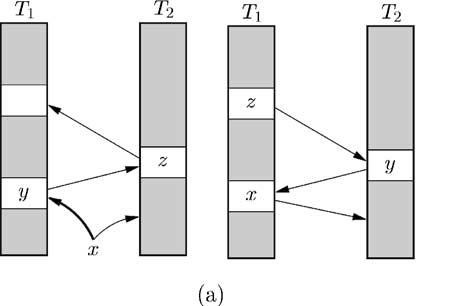
\includegraphics[width=0.4\linewidth]{cuckoo.jpg}
\end{figure}

\item Săgețile din fiecare cheie reprezintă pozițiile corespunzătoare acestora în tabelele T1 și T2.
\end{itemize}
\end{frame}
%------------------------------------------------
\begin{frame}[fragile]
\frametitle{Inserarea unei chei}
\begin{block}{Funcția de inserare}
\lstset{language = Python, 
        showstringspaces=false,
        basicstyle=\ttfamily\small,
        keywordstyle=\color{blue},
        }
\begin{lstlisting}
  def insert(x):
  	# Verificam daca cheia exista deja.
  	if lookup(x):
  		return
   	for i in range(MaxLoop):
   	  T1[h1[x]], x = x, T1[h1[x]]
   	  if x == None:
   	    return
   	  T2[h2[x]], x = x, T2[h2[x]]
   	  if x == None:
   	    return
   	# Daca nu am putut face inserarea
   	rehash()
   	insert(x)
\end{lstlisting}
\end{block}

\end{frame}
%------------------------------------------------
\begin{frame}
\frametitle{Variante de implementare}
\begin{itemize}
\item Se pot elabora diferite variante de implementare a acestui algoritm plecând de la diferite observații.

\item O primă variantă are la bază observația că algoritmul incearcă întâi să insereze în tabela T1. Din acest motiv putem folosi tabele de dimensiuni \textbf{asimetrice}, crescând dimensiunea tabelei T1.

\item O altă variantă este aceea de a folosi o singură tabela T de dimensiune $2r$ pentru ambele functii de hashing.

\begin{block}{Observație}
Pentru eleganță ultimei variante putem considera ca poziții fezabile pentru $x$ locațiile $h_1(x), (h_2(x) - h_1(x)) \mod 2r$. În acest mod putem sări de la o locație la alta folosind funcția $i \to (h_2(x) - i) \mod 2r$. Acest lucru se poate verifica ușor înlocuind pe i cu fiecare din locațiile posibile pentru $x$.
\end{block}

\end{itemize}
\end{frame}
%------------------------------------------------
\begin{frame}
\frametitle{Analiza complexității}
\begin{itemize}
\item Deoarece am concluzionat că operățiile de inserare și ștergere au o complexitate timp de $\mathcal{O}(1)$ vom analiza în cele ce urmează comportamentul operației de inserare care nu este unul trivial.

\begin{lemma}[]
\footnote{Demonstrația este una complexă și nu face subiectul acestei prezentări.}
Presupunem că procedura de inserare nu intră într-un ciclu infinit. Atunci pentru orice prefix $x_1, x_2, ..., x_p$ al secvenței de chei mutate de către procedură, există o secvența de \textbf{cel puțin $\frac{p}{3}$} chei consecutive fară repetiții, începând cu cheia $x_1$.
\end{lemma}.

\end{itemize}
\end{frame}
%------------------------------------------------
\begin{frame}
\frametitle{Analiza complexității}
\begin{itemize}

\item Lucrarea demonstrează ca probabilitatea de a cauza apelarea procedurii de rehash este de $\mathcal{O}(1/n^2)$

\item În particular fiecare operație de inserție ce este efectuată în cadrul procedurii de rehashing are o probabilitate de succes de $1 - \mathcal{O}(1/n)$

\item Obținem un timp mediu pentru procedura de rehashing de complexitate $\mathcal{O}(n)$ 

\item În cele din urmă combinând primul și al treilea rezultat reiese că pentru fiecare inserție timpul mediu pentru rehashing este de $\mathcal{O}(1/n)$, considerând șî apelare forțată a procedurii de rehashing o dată la $r^2$ inserări.

\item În concluzie am arătat că acest algoritm prezintă o complexitate $\mathcal{O}(1)$ amortizat pentru operația de inserare.
\end{itemize}
\end{frame}
%------------------------------------------------

\begin{frame}
\frametitle{Benchmarking}
\begin{table}
\begin{tabular}{l l l}
\toprule
\textbf{Treatments} & \textbf{Response 1} & \textbf{Response 2}\\
\midrule
Treatment 1 & 0.0003262 & 0.562 \\
Treatment 2 & 0.0015681 & 0.910 \\
Treatment 3 & 0.0009271 & 0.296 \\
\bottomrule
\end{tabular}
\caption{Table caption}
\end{table}
\end{frame}
%------------------------------------------------
\begin{frame}
\frametitle{Concluzii}
\begin{itemize}

\item Am prezentat un algoritm cu complexitate constantă în timp pentru cazul cel mai rău.

\item Algoritmul este unul elegant și simplu de implementat, prezentând mai multe variante ale acestuia.

\item Algoritmul se comportă excelent în practică.

\end{itemize}
\end{frame}
%------------------------------------------------

\begin{frame}
\frametitle{Referințe}
\footnotesize{
\begin{thebibliography}{99} % Beamer does not support BibTeX so references must be inserted manually as below
\bibitem[cuckoo]{p1} John Smith (2012)
\newblock Cuckoo Hashing
\newblock \emph{Journal of Algorithms} 51(2004), 122 -- 144.
\end{thebibliography}
}
\end{frame}

%------------------------------------------------

\begin{frame}
\Huge{\centerline{Mulțumesc}}
\end{frame}

%----------------------------------------------------------------------------------------

\end{document} 